\documentclass[aspectratio=169]{beamer}

% Page setup and packages
\usepackage[utf8]{inputenc}
\usepackage{amsmath}
\usepackage{amssymb}
\usepackage{booktabs}
\usepackage{graphicx}
\usepackage{hyperref}
\usepackage{color}
\usepackage{xcolor}

% Custom premium color palette
\definecolor{primary}{RGB}{15, 23, 42}      % Deep Slate/Blue
\definecolor{accent}{RGB}{14, 116, 144}     % Cyan/Teal Accent
\definecolor{secondary}{RGB}{124, 58, 237}  % Violet/Purple
\definecolor{textdark}{RGB}{30, 41, 59}     % Dark Gray Body Text
\definecolor{bglight}{RGB}{248, 250, 252}   % Off-white Slate
\definecolor{emerald}{RGB}{16, 185, 129}   % Soft Success Green
\definecolor{coral}{RGB}{239, 68, 68}      % Soft Error Red

% Beamer Theme Customization
\usetheme{Boadilla}
\usecolortheme{default}
\useinnertheme{rounded}

% Color settings for Beamer elements
\setbeamercolor{structure}{fg=accent}
\setbeamercolor{palette primary}{bg=primary, fg=white}
\setbeamercolor{palette secondary}{bg=secondary, fg=white}
\setbeamercolor{palette tertiary}{bg=accent, fg=white}
\setbeamercolor{palette quaternary}{bg=primary, fg=white}
\setbeamercolor{title}{fg=primary}
\setbeamercolor{frametitle}{bg=primary, fg=white}
\setbeamercolor{block title}{bg=primary, fg=white}
\setbeamercolor{block body}{bg=bglight, fg=textdark}
\setbeamercolor{block title alerted}{bg=coral, fg=white}
\setbeamercolor{block body alerted}{bg=bglight, fg=textdark}
\setbeamercolor{block title example}{bg=emerald, fg=white}
\setbeamercolor{block body example}{bg=bglight, fg=textdark}

% Customizing fonts
\usefonttheme{professionalfonts}
\setbeamerfont{title}{size=\Large, series=\bfseries}
\setbeamerfont{subtitle}{size=\small, shape=\itshape}
\setbeamerfont{frametitle}{size=\large, series=\bfseries}

% Remove navigation symbols
\setbeamertemplate{navigation symbols}{}

% Document Information
\title[VLM Cross-Task Contradictions]{Know It's Absent, Yet Point Anyway}
\subtitle{Cross-Task Semantic Contradictions in Vision-Language Models}
\author[Bac, My, Phuong]{Presented by:\\Nguyen Ba Thanh Bac; Nguyen Thi Tra My; Tran Thi Hoai Phuong}
\institute{NLP Course Presentation (2025/2026)}
\date{\today}

\begin{document}

% Slide 1: Title Slide
\begin{frame}[plain]
    \titlepage
\end{frame}

% Slide 2: Introduction & Motivation
\begin{frame}{Introduction \& Motivation}
    \begin{columns}[T]
        \begin{column}{0.48\textwidth}
            \begin{block}{Rapid Rise of Multimodal NLP}
                Vision-Language Models (VLMs) have revolutionized multimodal NLP, combining:
                \begin{itemize}
                    \item Generative NLP reasoning
                    \item Visual Question Answering (VQA)
                    \item Spatial Grounding (connecting text tokens to pixel coordinates/bounding boxes)
                \end{itemize}
            \end{block}
        \end{column}
        
        \begin{column}{0.48\textwidth}
            \begin{alertblock}{The Semantic Consistency Challenge}
                Despite high VQA performance, VLMs exhibit severe \textbf{cross-task logical inconsistencies}:
                \begin{itemize}
                    \item They correctly recognize object absence in text format...
                    \item ...yet fail to preserve this semantic judgment when the task is reformulated as a grounding prompt.
                \end{itemize}
            \end{alertblock}
        \end{column}
    \end{columns}
    
    \vspace{0.2cm}
    \centering
    \textcolor{secondary}{\textbf{Key Question:}} How can a model that correctly answers ``No'' to ``Is there a cat?'' still draw a bounding box when later asked to ``Point to the cat''?
\end{frame}

% Slide 3: Part 1 - The Phenomenon (Tailored to NLP reasoning & agents)
\begin{frame}{Part 1: The Phenomenon -- Existence-Localization Contradiction}
    \begin{columns}[T]
        \begin{column}{0.48\textwidth}
            \begin{block}{The Core Contradiction}
                A systematic failure mode where a VLM:
                \begin{enumerate}
                    \item Correctly recognizes that a queried object is \textbf{absent} from an image,
                    \item But still produces a \textbf{non-null, hallucinated localization} (bounding box) when asked to ground the same referent.
                \end{enumerate}
                This isolates cases where models know the referent is absent but fail to carry this judgment into grounding.
            \end{block}
        \end{column}
        
        \begin{column}{0.48\textwidth}
            \begin{alertblock}{Actionable Hallucination in NLP Agents}
                A physical grounding commitment contradicts the internal semantic belief.
                \begin{itemize}
                    \item Critical for \textbf{downstream NLP systems} (grounding-based tool use, database retrieval, multimodal web agents).
                    \item Propagates false evidence, triggering incorrect downstream actions in multimodal pipelines.
                \end{itemize}
            \end{alertblock}
        \end{column}
    \end{columns}
\end{frame}

% Slide 4: Part 1 - Concrete Example (Figure 1)
\begin{frame}{Part 1: A Concrete Example (Figure 1)}
    \begin{center}
        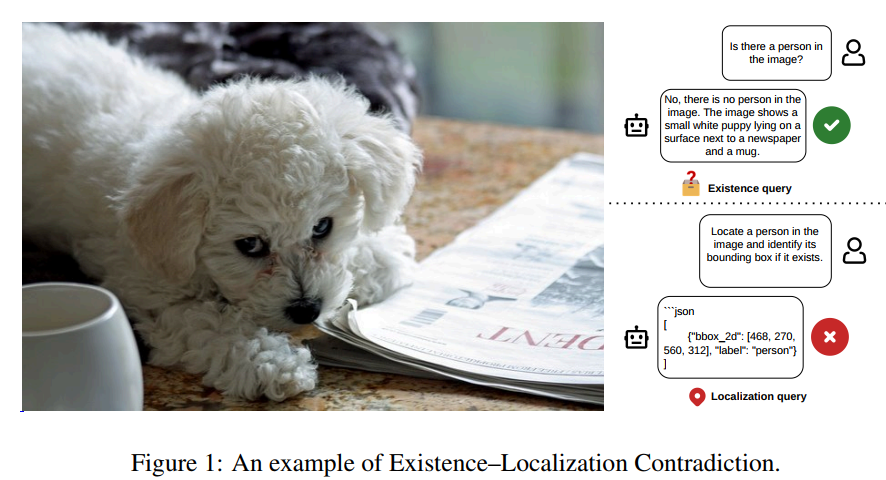
\includegraphics[width=0.82\textwidth]{figure1.png}
    \end{center}
    \vspace{-0.2cm}
    \centering \small \textit{Figure 1: VLM correctly recognizes object absence in VQA but localizes it anyway when prompted.}
\end{frame}

% Slide 5: Part 1 - Conditional Evaluation Protocol
\begin{frame}{Part 1: Measuring Contradictions -- Conditional Protocol}
    \begin{columns}[T]
        \begin{column}{0.5\textwidth}
            \begin{block}{2-Stage Conditional Protocol}
                To isolate contradictions, the authors evaluate localization \textbf{only} when the model correctly identifies absence:
                \vskip 0.15cm
                \textbf{Stage 1: Existence Recognition}
                \begin{itemize}
                    \item Query VLM with existence prompt $T_E(o_i)$ on negative set (absent objects).
                    \item Filter cases with correct absence ($\hat{e}_i = 0$).
                \end{itemize}
                \textbf{Stage 2: Localization under Absence}
                \begin{itemize}
                    \item Query the VLM with localization prompt $T_L(o_i)$.
                    \item Assess if it returns a null output ($\hat{\ell}_i = 0$).
                \end{itemize}
            \end{block}
        \end{column}
        
        \begin{column}{0.46\textwidth}
            \begin{exampleblock}{Primary Metric: CELF}
                \textbf{Conditional Existence-Localization Faithfulness (CELF)}:
                \begin{equation*}
                    \text{CELF} = \Pr(\hat{\ell}_i = 0 \mid e_i = 0, \hat{e}_i = 0)
                \end{equation*}
                \vskip 0.1cm
                CELF measures how often the model remains faithful to its prior correct absence judgment during localization.
                \begin{itemize}
                    \item \textbf{CELF = 1.0:} Perfect consistency.
                    \item \textbf{CELF = 0.0:} Complete failure (always localizes anyway).
                \end{itemize}
            \end{exampleblock}
        \end{column}
    \end{columns}
\end{frame}

% Slide 6: Part 2 - Analysis & Observations (Base Results)
\begin{frame}{Part 2: Prevalence of Contradictions in Strong VLMs}
    \begin{columns}[T]
        \begin{column}{0.58\textwidth}
            \begin{table}
                \centering
                \footnotesize
                \caption{Baseline CELF results on POPE, AMBER, MME, DASH-B}
                \begin{tabular}{llcccc}
                    \toprule
                    \textbf{Model} & \textbf{Metric} & \textbf{POPE} & \textbf{AMB} & \textbf{MME} & \textbf{DASH} \\
                    \midrule
                    Qwen2.5-7B   & EA $\uparrow$ & 83.7\% & 95.4\% & 100\% & 74.3\% \\
                                 & \textbf{CELF} $\uparrow$ & \textbf{10.4\%} & \textbf{28.6\%} & \textbf{20.0\%} & \textbf{2.8\%} \\
                    \midrule
                    Qwen3-8B     & EA $\uparrow$ & 89.4\% & 90.2\% & 98.3\% & 74.5\% \\
                                 & \textbf{CELF} $\uparrow$ & \textbf{15.8\%} & \textbf{38.2\%} & \textbf{50.0\%} & \textbf{2.7\%} \\
                    \midrule
                    InternVL3    & EA $\uparrow$ & 90.8\% & 92.3\% & 98.3\% & 67.6\% \\
                                 & \textbf{CELF} $\uparrow$ & \textbf{0.0\%} & \textbf{0.0\%} & \textbf{0.0\%} & \textbf{0.0\%} \\
                    \bottomrule
                \end{tabular}
            \end{table}
        \end{column}
        
        \begin{column}{0.38\textwidth}
            \begin{alertblock}{Key Observation}
                While Existence Accuracy (EA) is consistently high ($80\% - 100\%$), \textbf{CELF scores are strikingly low}. 
                \vskip 0.15cm
                InternVL models achieve \textbf{0.0\% CELF} across all datasets, meaning they \textbf{never abstain} under localization queries, even when they just correctly recognized object absence.
            \end{alertblock>
        \end{column}
    \end{columns}
\end{frame}

% Slide 7: Part 2 - Hidden Space Analysis (Representation Probing in VLM)
\begin{frame}{Part 2: Representation Probing -- Why Do Contradictions Occur?}
    \begin{columns}[T]
        \begin{column}{0.48\textwidth}
            \begin{center}
                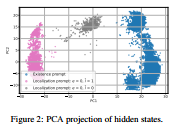
\includegraphics[width=0.92\textwidth]{figure2.png}
            \end{center}
            \vspace{-0.1cm}
            \centering \scriptsize \textit{Figure 2: PCA projection of hidden states at the final token position.}
        \end{column}
        
        \begin{column}{0.48\textwidth}
            \begin{block}{Task Representation Separation}
                \small
                \begin{itemize}
                    \item Hidden states under \textbf{existence prompts} and \textbf{localization prompts} form two highly distinct clusters.
                    \item Represents different internal ``regimes'' with very limited multi-task knowledge sharing.
                \end{itemize}
            \end{block}
            \begin{exampleblock}{Proximity of Correct Rejections}
                \small
                \begin{itemize}
                    \item Correct null-localizations lie significantly \textbf{closer} to the existence prompt cluster.
                    \item Rejection succeeds when the VLM manages to leverage prior existence knowledge.
                \end{itemize}
            \end{exampleblock}
        \end{column}
    \end{columns}
\end{frame}

% Slide 8: Part 3 - Solution (Tailored to Activation Engineering in LLMs)
\begin{frame}{Part 3: Solution -- Representation Steering (Activation Engineering)}
    The authors propose \textbf{inference-time activation steering} to shift hidden states towards absence-consistent representations (Parameter-Free, localized, and efficient):
    
    \vspace{0.1cm}
    \begin{block}{Step-by-Step Methodology}
        \small
        \begin{enumerate}
            \item \textbf{Paired Contrastive Set:} Build a set $\mathcal{P}$ of 100 examples. For each query, extract hidden states at transformer layer $l$ for the hallucinated response $h_{loc}^{(l)}$ and the correct abstention response $h_{abs}^{(l)}$.
            \item \textbf{Compute Steering Direction Vector ($s^{(l)}$):} Define the mean difference vector (similar to LLM truthfulness steering):
                  \begin{equation*}
                      s^{(l)} = \frac{1}{M} \sum_{i=1}^M \left( h_{i, abs}^{(l)} - h_{i, loc}^{(l)} \right)
                  \end{equation*}
            \item \textbf{Inference-Time Injection:} Add the steering vector into the hidden representation during test time at layer $l$:
                  \begin{equation*}
                      \tilde{h}^{(l)} = h^{(l)} + \alpha s^{(l)}
                  \end{equation*}
        \end{enumerate}
    \end{block}
\end{frame}

% Slide 9: Part 3 - Results after Steering (Figure 3)
\begin{frame}{Part 3: CELF Performance under Different Steering Scales}
    \begin{center}
        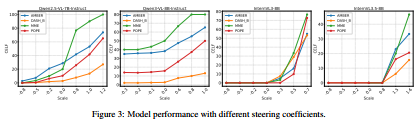
\includegraphics[width=0.86\textwidth]{figure3.png}
    \end{center}
    \vspace{-0.2cm}
    \centering \small \textit{Figure 3: Model performance (CELF metric) increases steadily as positive steering scale $\alpha$ rises.}
\end{frame}

% Slide 10: Conclusion (NLP Core Perspectives)
\begin{frame}{Conclusion \& Outlook}
    \begin{columns}[T]
        \begin{column}{0.48\textwidth}
            \begin{block}{Summary of Contributions}
                \small
                \begin{itemize}
                    \item \textbf{Identified Contradiction:} Uncovered Existence-Localization Contradiction as a systematic semantic logic failure in leading VLMs.
                    \item \textbf{Conditional Protocol:} Formulated the CELF metric to evaluate consistency.
                    \item \textbf{Activation Steering:} Demonstrated that lightweight activation steering dramatically restores absence-consistent grounding.
                \end{itemize}
            \end{block}
        \end{column}
        
        \begin{column}{0.48\textwidth}
            \begin{exampleblock}{NLP Research Perspectives}
                \small
                \begin{itemize}
                    \item \textbf{Interpretable NLP:} Highlights the power of representation probing and steering to dynamically align VLM behaviors without fine-tuning.
                    \item \textbf{Architectural Coherence:} Encourages designing multi-task pretraining or loss formulations that bind text reasoning and spatial grounding logic, rather than treating them as isolated tasks.
                \end{itemize}
            \end{exampleblock}
        \end{column}
    \end{columns}
\end{frame}

\end{document}
